\documentclass[tikz,border=4pt]{standalone}
\usepackage[T1]{fontenc}
\usepackage[utf8]{inputenc}
\usepackage{amsmath,amssymb}
\usepackage{helvet}
\renewcommand{\familydefault}{\sfdefault}
\usepackage{pgfplots}
\pgfplotsset{compat=1.17}
\usetikzlibrary{arrows.meta,positioning,calc,fit,backgrounds,shapes.geometric}

\definecolor{cVis}{HTML}{1F77B4}
\definecolor{cTxt}{HTML}{D62728}
\definecolor{cProj}{HTML}{2CA02C}
\definecolor{cLLM}{HTML}{9467BD}
\definecolor{cConv}{HTML}{FF7F0E}
\definecolor{cAtt}{HTML}{17BECF}
\definecolor{cGray}{HTML}{7F7F7F}

\tikzset{
  blk/.style={draw, rounded corners=2pt, minimum height=8mm, align=center, font=\footnotesize, thick},
  tok/.style={draw, minimum size=3.2mm, inner sep=0pt},
  arr/.style={-{Stealth[length=2mm]}, thick},
}

\begin{document}
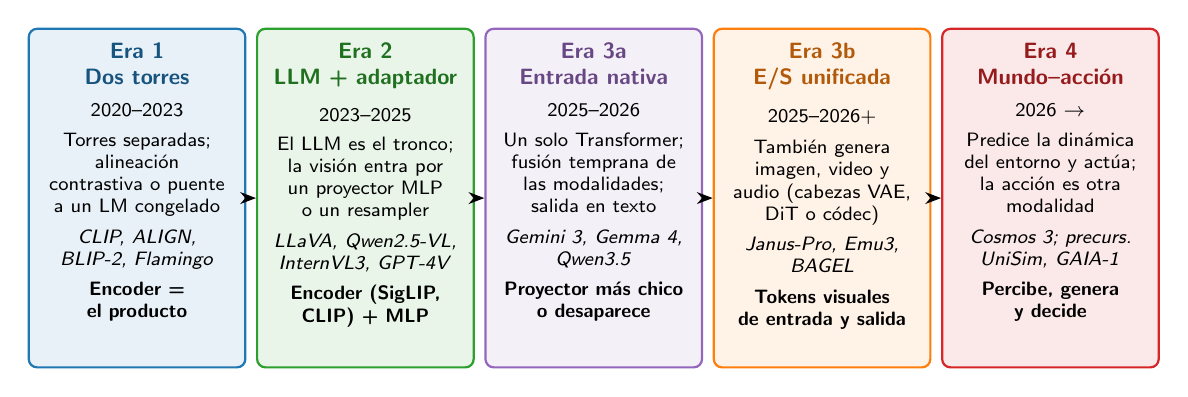
\begin{tikzpicture}[
    era/.style={draw, rounded corners=3pt, thick, minimum width=27.5mm, minimum height=43mm, anchor=north},
    hd/.style={font=\footnotesize\bfseries, align=center}]
  \foreach \x/\c/\t/\y/\body [count=\k] in {
    0/cVis/{Era 1\\Dos torres}/{2020--2023}/{Torres separadas;\\alineación\\contrastiva o puente\\a un LM congelado\\[3pt]\textit{CLIP, ALIGN,}\\\textit{BLIP-2, Flamingo}\\[3pt]\textbf{Encoder =}\\\textbf{el producto}},
    2.9/cProj/{Era 2\\LLM + adaptador}/{2023--2025}/{El LLM es el tronco;\\la visión entra por\\un proyector MLP\\o un resampler\\[3pt]\textit{LLaVA, Qwen2.5-VL,}\\\textit{InternVL3, GPT-4V}\\[3pt]\textbf{Encoder (SigLIP,}\\\textbf{CLIP) + MLP}},
    5.8/cLLM/{Era 3a\\Entrada nativa}/{2025--2026}/{Un solo Transformer;\\fusión temprana de\\las modalidades;\\salida en texto\\[3pt]\textit{Gemini 3, Gemma 4,}\\\textit{Qwen3.5}\\[3pt]\textbf{Proyector más chico}\\\textbf{o desaparece}},
    8.7/cConv/{Era 3b\\E/S unificada}/{2025--2026+}/{También genera\\imagen, video y\\audio (cabezas VAE,\\DiT o códec)\\[3pt]\textit{Janus-Pro, Emu3,}\\\textit{BAGEL}\\[3pt]\textbf{Tokens visuales}\\\textbf{de entrada y salida}},
    11.6/cTxt/{Era 4\\Mundo–acción}/{2026 $\to$}/{Predice la dinámica\\del entorno y actúa;\\la acción es otra\\modalidad\\[3pt]\textit{Cosmos 3; precurs.}\\\textit{UniSim, GAIA-1}\\[3pt]\textbf{Percibe, genera}\\\textbf{y decide}}}{
    \node[era, fill=\c!10, draw=\c] (e\k) at (\x,0) {};
    \node[hd, text=\c!70!black, below=2pt of e\k.north] (h\k) {\t};
    \node[font=\scriptsize, below=0pt of h\k] (y\k) {\y};
    \node[font=\scriptsize, align=center, below=2pt of y\k, inner sep=0pt] {\body};
  }
  \foreach \a/\b in {1/2,2/3,3/4,4/5}{\draw[arr] (e\a.east) -- (e\b.west);}
\end{tikzpicture}
\end{document}
